% Options for packages loaded elsewhere
\PassOptionsToPackage{unicode}{hyperref}
\PassOptionsToPackage{hyphens}{url}
\PassOptionsToPackage{dvipsnames,svgnames*,x11names*}{xcolor}
%
\documentclass[
  10pt,
]{article}
\usepackage{amsmath,amssymb}
\usepackage{lmodern}
\usepackage{iftex}
\ifPDFTeX
  \usepackage[T1]{fontenc}
  \usepackage[utf8]{inputenc}
  \usepackage{textcomp} % provide euro and other symbols
\else % if luatex or xetex
  \usepackage{unicode-math}
  \defaultfontfeatures{Scale=MatchLowercase}
  \defaultfontfeatures[\rmfamily]{Ligatures=TeX,Scale=1}
  \setmainfont[]{Charter}
  \setmonofont[Scale=0.80]{Menlo}
\fi
% Use upquote if available, for straight quotes in verbatim environments
\IfFileExists{upquote.sty}{\usepackage{upquote}}{}
\IfFileExists{microtype.sty}{% use microtype if available
  \usepackage[]{microtype}
  \UseMicrotypeSet[protrusion]{basicmath} % disable protrusion for tt fonts
}{}
\makeatletter
\@ifundefined{KOMAClassName}{% if non-KOMA class
  \IfFileExists{parskip.sty}{%
    \usepackage{parskip}
  }{% else
    \setlength{\parindent}{0pt}
    \setlength{\parskip}{6pt plus 2pt minus 1pt}}
}{% if KOMA class
  \KOMAoptions{parskip=half}}
\makeatother
\usepackage{xcolor}
\IfFileExists{xurl.sty}{\usepackage{xurl}}{} % add URL line breaks if available
\IfFileExists{bookmark.sty}{\usepackage{bookmark}}{\usepackage{hyperref}}
\hypersetup{
  colorlinks=true,
  linkcolor={RoyalBlue},
  filecolor={Maroon},
  citecolor={Blue},
  urlcolor={RoyalBlue},
  pdfcreator={LaTeX via pandoc}}
\urlstyle{same} % disable monospaced font for URLs
\usepackage[margin=0.9in]{geometry}
\usepackage{color}
\usepackage{fancyvrb}
\newcommand{\VerbBar}{|}
\newcommand{\VERB}{\Verb[commandchars=\\\{\}]}
\DefineVerbatimEnvironment{Highlighting}{Verbatim}{commandchars=\\\{\}}
% Add ',fontsize=\small' for more characters per line
\usepackage{framed}
\definecolor{shadecolor}{RGB}{248,248,248}
\newenvironment{Shaded}{\begin{snugshade}}{\end{snugshade}}
\newcommand{\AlertTok}[1]{\textcolor[rgb]{0.94,0.16,0.16}{#1}}
\newcommand{\AnnotationTok}[1]{\textcolor[rgb]{0.56,0.35,0.01}{\textbf{\textit{#1}}}}
\newcommand{\AttributeTok}[1]{\textcolor[rgb]{0.77,0.63,0.00}{#1}}
\newcommand{\BaseNTok}[1]{\textcolor[rgb]{0.00,0.00,0.81}{#1}}
\newcommand{\BuiltInTok}[1]{#1}
\newcommand{\CharTok}[1]{\textcolor[rgb]{0.31,0.60,0.02}{#1}}
\newcommand{\CommentTok}[1]{\textcolor[rgb]{0.56,0.35,0.01}{\textit{#1}}}
\newcommand{\CommentVarTok}[1]{\textcolor[rgb]{0.56,0.35,0.01}{\textbf{\textit{#1}}}}
\newcommand{\ConstantTok}[1]{\textcolor[rgb]{0.00,0.00,0.00}{#1}}
\newcommand{\ControlFlowTok}[1]{\textcolor[rgb]{0.13,0.29,0.53}{\textbf{#1}}}
\newcommand{\DataTypeTok}[1]{\textcolor[rgb]{0.13,0.29,0.53}{#1}}
\newcommand{\DecValTok}[1]{\textcolor[rgb]{0.00,0.00,0.81}{#1}}
\newcommand{\DocumentationTok}[1]{\textcolor[rgb]{0.56,0.35,0.01}{\textbf{\textit{#1}}}}
\newcommand{\ErrorTok}[1]{\textcolor[rgb]{0.64,0.00,0.00}{\textbf{#1}}}
\newcommand{\ExtensionTok}[1]{#1}
\newcommand{\FloatTok}[1]{\textcolor[rgb]{0.00,0.00,0.81}{#1}}
\newcommand{\FunctionTok}[1]{\textcolor[rgb]{0.00,0.00,0.00}{#1}}
\newcommand{\ImportTok}[1]{#1}
\newcommand{\InformationTok}[1]{\textcolor[rgb]{0.56,0.35,0.01}{\textbf{\textit{#1}}}}
\newcommand{\KeywordTok}[1]{\textcolor[rgb]{0.13,0.29,0.53}{\textbf{#1}}}
\newcommand{\NormalTok}[1]{#1}
\newcommand{\OperatorTok}[1]{\textcolor[rgb]{0.81,0.36,0.00}{\textbf{#1}}}
\newcommand{\OtherTok}[1]{\textcolor[rgb]{0.56,0.35,0.01}{#1}}
\newcommand{\PreprocessorTok}[1]{\textcolor[rgb]{0.56,0.35,0.01}{\textit{#1}}}
\newcommand{\RegionMarkerTok}[1]{#1}
\newcommand{\SpecialCharTok}[1]{\textcolor[rgb]{0.00,0.00,0.00}{#1}}
\newcommand{\SpecialStringTok}[1]{\textcolor[rgb]{0.31,0.60,0.02}{#1}}
\newcommand{\StringTok}[1]{\textcolor[rgb]{0.31,0.60,0.02}{#1}}
\newcommand{\VariableTok}[1]{\textcolor[rgb]{0.00,0.00,0.00}{#1}}
\newcommand{\VerbatimStringTok}[1]{\textcolor[rgb]{0.31,0.60,0.02}{#1}}
\newcommand{\WarningTok}[1]{\textcolor[rgb]{0.56,0.35,0.01}{\textbf{\textit{#1}}}}
\usepackage{longtable,booktabs,array}
\usepackage{calc} % for calculating minipage widths
% Correct order of tables after \paragraph or \subparagraph
\usepackage{etoolbox}
\makeatletter
\patchcmd\longtable{\par}{\if@noskipsec\mbox{}\fi\par}{}{}
\makeatother
% Allow footnotes in longtable head/foot
\IfFileExists{footnotehyper.sty}{\usepackage{footnotehyper}}{\usepackage{footnote}}
\makesavenoteenv{longtable}
\usepackage{graphicx}
\makeatletter
\def\maxwidth{\ifdim\Gin@nat@width>\linewidth\linewidth\else\Gin@nat@width\fi}
\def\maxheight{\ifdim\Gin@nat@height>\textheight\textheight\else\Gin@nat@height\fi}
\makeatother
% Scale images if necessary, so that they will not overflow the page
% margins by default, and it is still possible to overwrite the defaults
% using explicit options in \includegraphics[width, height, ...]{}
\setkeys{Gin}{width=\maxwidth,height=\maxheight,keepaspectratio}
% Set default figure placement to htbp
\makeatletter
\def\fps@figure{htbp}
\makeatother
\setlength{\emergencystretch}{3em} % prevent overfull lines
\providecommand{\tightlist}{%
  \setlength{\itemsep}{0pt}\setlength{\parskip}{0pt}}
\setcounter{secnumdepth}{-\maxdimen} % remove section numbering
\ifLuaTeX
  \usepackage{selnolig}  % disable illegal ligatures
\fi

\title{USRP B210 SDR Link — System Reference}
\author{}
\date{}

\begin{document}
\maketitle

{
\hypersetup{linkcolor=}
\setcounter{tocdepth}{3}
\tableofcontents
}
\hypertarget{usrp-b210-sdr-link--system-reference}{%
\section{USRP B210 SDR Link --- System
Reference}\label{usrp-b210-sdr-link--system-reference}}

End-to-end digital communication system for two USRP B210 radios (UHD),
written in C++. This document lists \textbf{every feature, algorithm
(with the math and the common alternatives), and command-line option}
exposed by \texttt{sdr\_system}.

\begin{itemize}
\tightlist
\item
  Binary: \texttt{build/sdr\_system}
\item
  Help: \texttt{./sdr\_system\ -\/-help}
\item
  Two operating styles: \textbf{one-way} (\texttt{-\/-role\ tx} /
  \texttt{-\/-role\ rx}, repeated sends, auto-terminating RX) and
  \textbf{ARQ} (\texttt{-\/-role\ source\_arq} /
  \texttt{-\/-role\ sink\_arq}, stop-and-wait with ACK).
\end{itemize}

\begin{center}\rule{0.5\linewidth}{0.5pt}\end{center}

\hypertarget{1-signal-chain-overview}{%
\subsection{1. Signal-chain overview}\label{1-signal-chain-overview}}

\begin{verbatim}
TX:  message ─> split into chunks ─> CRC-16 ─> [FEC encode] ─> bits->symbols (modulator)
        ├── single-carrier: RRC pulse-shape ─> preamble prepend ─> USRP TX
        └── OFDM:            QAM->IFFT+CP frame [SC-sync | chan-est | data] ─> USRP TX

RX:  USRP RX ─> energy detector (burst gate) ─> AGC ─> frame/symbol sync
        ├── single-carrier: matched filter ─> timing (Gardner) ─> [equalizer] ─> demod
        └── OFDM:            Schmidl-Cox sync + CFO ─> FFT ─> 1-tap eq ─> pilot CPE ─> demod
     ─> [FEC decode] ─> CRC-16 check ─> (ARQ: ACK if OK) ─> reassemble message
\end{verbatim}

Default physical parameters: symbol rate \texttt{0.8\ MHz},
\texttt{U/D\ =\ 2/1} -\textgreater{} sample rate \texttt{1.6\ MHz}
(integer \textbf{2 samples/symbol} on the wire), RRC roll-off
\texttt{0.25}, 151 taps.

\begin{center}\rule{0.5\linewidth}{0.5pt}\end{center}

\hypertarget{2-modulation}{%
\subsection{2. Modulation}\label{2-modulation}}

\texttt{-\/-scheme\ \textless{}NAME\textgreater{}} selects the
constellation. Supported (bits/symbol in parentheses):

\begin{longtable}[]{@{}lll@{}}
\toprule
Family & Schemes & bits/sym \\
\midrule
\endhead
PSK & \texttt{BPSK} (1), \texttt{QPSK} (2), \texttt{8-PSK} (3) & 1--3 \\
QAM & \texttt{16-QAM} (4), \texttt{32-QAM} (5), \texttt{64-QAM} (6),
\texttt{128-QAM} (7), \texttt{256-QAM} (8) & 4--8 \\
Differential & \texttt{DBPSK} (1), \texttt{DQPSK} (2), \texttt{8-DPSK}
(3), \texttt{PI4-QPSK} (2) & 1--3 \\
APSK & \texttt{16APSK} (4), \texttt{32APSK} (5) & 4--5 \\
\bottomrule
\end{longtable}

(\texttt{16QAM} and \texttt{16-QAM} spellings both accepted.)

\textbf{Math.} A modulator maps \(k=\log_2 M\) bits to one of \(M\)
complex points \(s = I + jQ\):

\begin{itemize}
\tightlist
\item
  \textbf{M-PSK}: points on the unit circle, \(s = e^{\,j2\pi m/M}\),
  \(m=0,\dots,M-1\). All symbols equal-energy; demod by nearest angle.
  Robust but spectrally inefficient at high order (points crowd on the
  circle).
\item
  \textbf{M-QAM}: square/cross grid of amplitudes,
  \(s = (2i-\sqrt{M}+1) + j\,(2q-\sqrt{M}+1)\). Best power efficiency
  for a given rate on an AWGN channel, but needs accurate amplitude
  -\textgreater{} sensitive to gain/EVM/clipping (this is why 16-QAM
  failed OTA at \textasciitilde20 \% EVM while QPSK survived
  \textasciitilde37 \%).
\item
  \textbf{APSK}: points on a few concentric rings. Lower PAPR than QAM,
  favored on non-linear (satellite) amplifiers --- a middle ground
  between PSK and QAM.
\item
  \textbf{Differential (D*)}: information is in the \textbf{phase
  change} between consecutive symbols,
  \(s_n = s_{n-1}\,e^{\,j\Delta\varphi}\). No absolute phase reference
  needed -\textgreater{} tolerates carrier phase offset / no PLL, at a
  \textasciitilde3 dB SNR penalty. \texttt{PI4-QPSK} rotates the
  constellation by \(\pi/4\) each symbol to avoid zero-crossings (lower
  envelope variation).
\end{itemize}

\textbf{Detection \& why constellation order costs SNR.} The demodulator
makes a \textbf{minimum-distance decision} --- pick the constellation
point nearest the received symbol \(y\) (optimal for equiprobable
symbols in AWGN):

\[ \hat{s} = \arg\min_{c\,\in\,\mathcal{C}} \; |\,y - c\,| \]

An error occurs when noise/distortion pushes \(y\) past the halfway line
to a neighbour, i.e. beyond half the \textbf{minimum distance}
\(d_{\min}/2\). For a fixed average power \(E_s\), packing more points
shrinks \(d_{\min}\): QPSK has \(d_{\min}=\sqrt{2E_s}\) with the whole
plane split into 4 quadrants, while 16-QAM squeezes 16 points into the
same power so \(d_{\min}\) is \textasciitilde3× smaller and its decision
cells \textasciitilde3× tighter. The \textbf{error vector magnitude}

\[ \mathrm{EVM} = \frac{\mathrm{rms}(\,y-\hat{s}\,)}{\mathrm{rms}(c)} \]

measures how far symbols land from ideal; reliable decoding needs
roughly \(\mathrm{EVM} \lesssim d_{\min}/(2\,\mathrm{rms})\), which is
why QPSK survived \textasciitilde37 \% EVM over the air but 16-QAM
(needing \(\lesssim 12\%\)) did not. \textbf{Gray coding} the
bit-\textgreater point map (adjacent points differ by one bit) makes
each symbol error cost only \textasciitilde1 bit error.

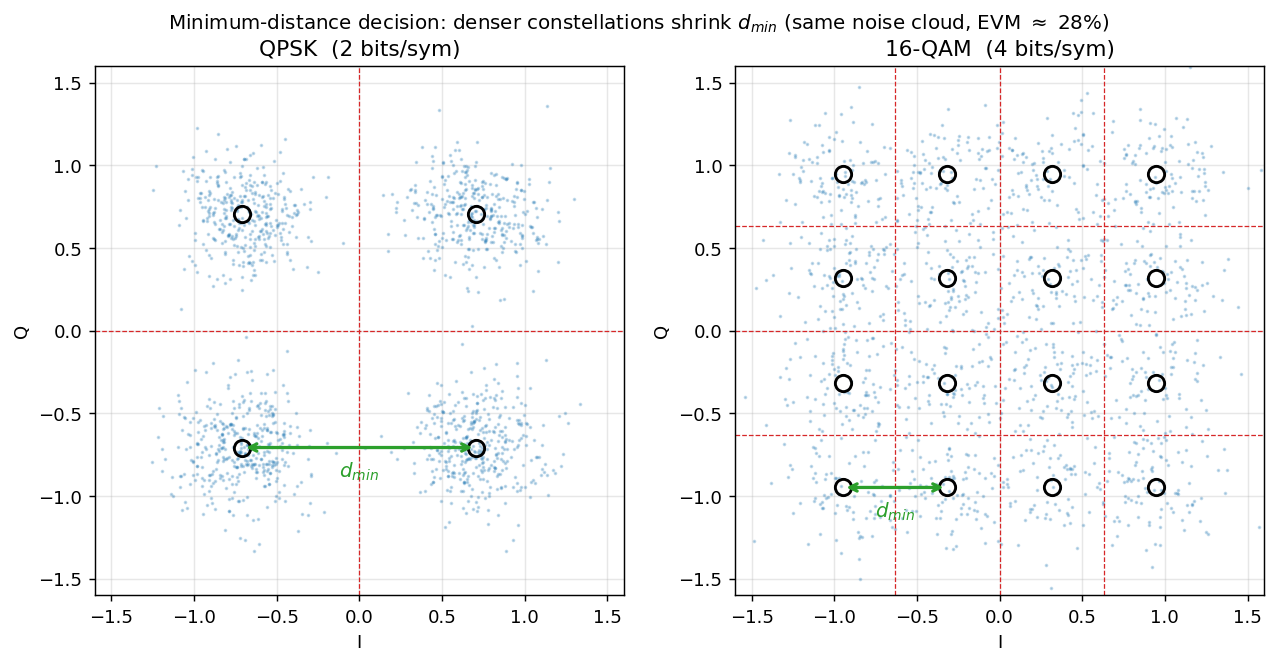
\includegraphics{figures/constellations.png}

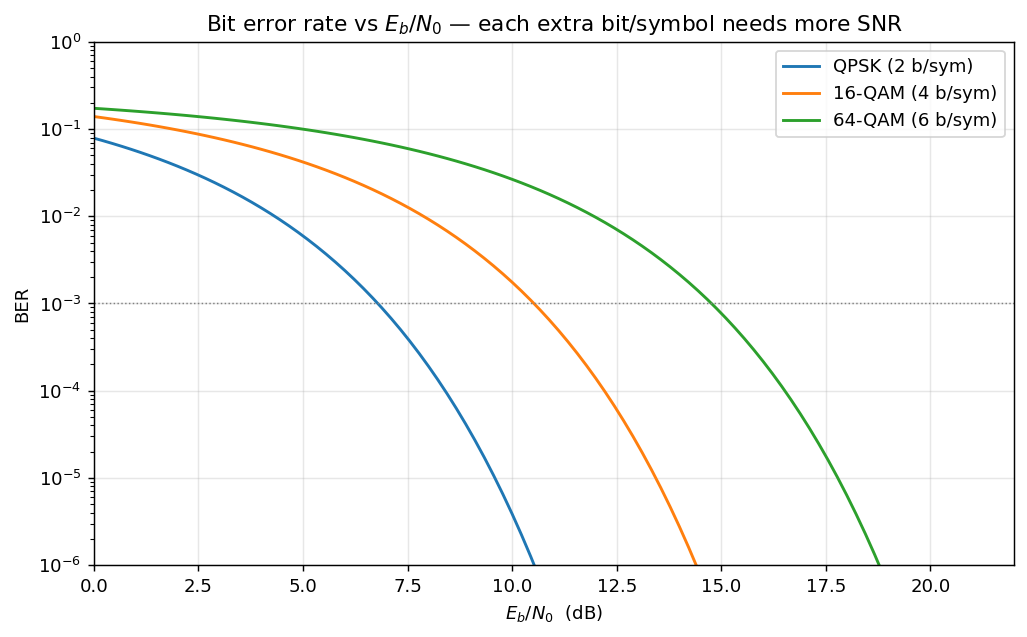
\includegraphics{figures/ber_curves.png}

\textbf{Bits\textless-\textgreater symbols detail.} Gray-like index
mapping; \texttt{bits\_to\_index} zero-fills a partial final group so
schemes whose bits/symbol don't divide the frame (32-QAM, 128-QAM) still
align --- a bug fixed early in this project.

\textbf{Common alternatives not implemented:} GMSK/CPM
(constant-envelope, used in GSM/Bluetooth), non-square 8-QAM,
probabilistic constellation shaping.

\begin{center}\rule{0.5\linewidth}{0.5pt}\end{center}

\hypertarget{3-waveform-single-carrier-vs-ofdm}{%
\subsection{3. Waveform: single-carrier vs
OFDM}\label{3-waveform-single-carrier-vs-ofdm}}

\texttt{-\/-waveform\ sc} (default) or \texttt{-\/-waveform\ ofdm}.

\hypertarget{31-single-carrier--rrc-pulse-shaping}{%
\subsubsection{3.1 Single-carrier + RRC pulse
shaping}\label{31-single-carrier--rrc-pulse-shaping}}

Symbols are upsampled \texttt{U/D} and convolved with a
\textbf{root-raised-cosine} filter (\texttt{-\/-filter\_type\ rrc},
\texttt{-\/-roll\_off\ 0.25}, \texttt{-\/-num\_taps\ 151}).

\textbf{Math.} A raised-cosine (RC) spectrum satisfies the
\textbf{Nyquist ISI criterion} --- its impulse response is zero at every
other symbol instant, \(g(mT)=\delta[m]\) --- so neighbouring symbols
don't interfere at the sampling times. Splitting it as \textbf{RRC at TX
and RRC at RX} makes the cascade \(G_{RRC}(f)\,G_{RRC}(f)=G_{RC}(f)\) a
full RC (matched-filter optimal in AWGN) \emph{and} maximizes SNR. The
roll-off \(\beta \in [0,1]\) trades occupied bandwidth against sidelobe
decay:

\[ B = (1+\beta)\,\frac{R_{sym}}{2}\quad\text{(one-sided baseband; occupied width }=(1+\beta)R_{sym}). \]

Alternatives: \texttt{rc} (raised cosine, all shaping at TX),
\texttt{lp} (plain low-pass); Gaussian shaping (GMSK) is the common
constant-envelope alternative.

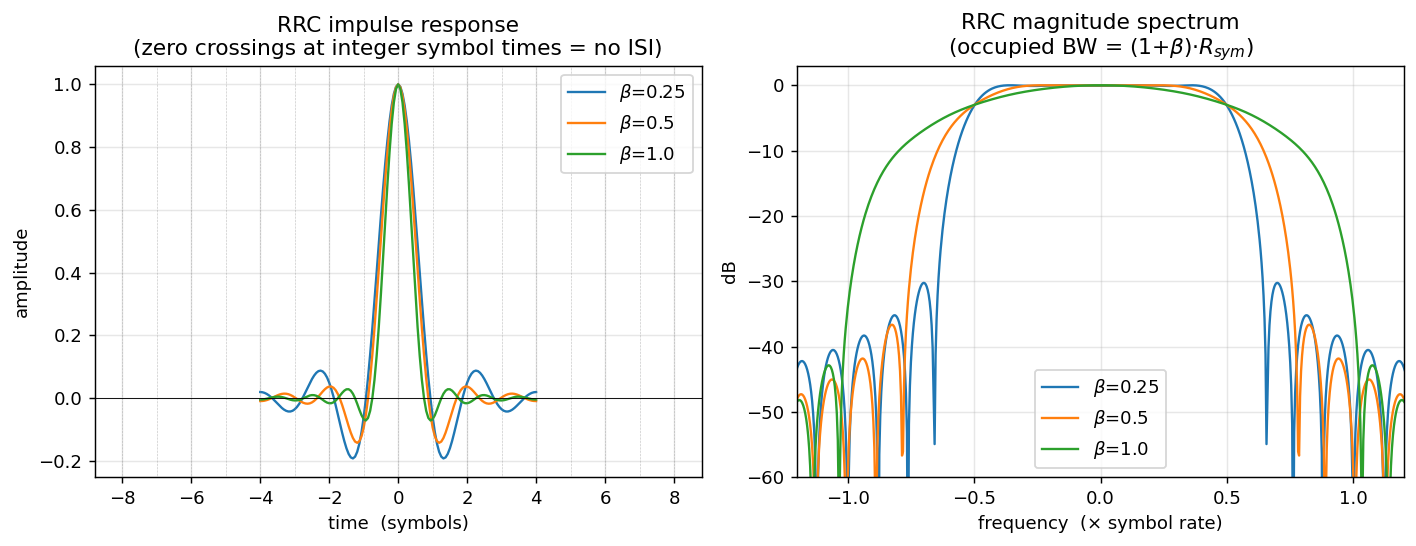
\includegraphics{figures/rrc.png}

\hypertarget{32-ofdm}{%
\subsubsection{3.2 OFDM}\label{32-ofdm}}

Frame layout per burst:
\texttt{{[}\ Schmidl-Cox\ sync\ symbol\ \textbar{}\ channel-estimation\ symbol\ \textbar{}\ data\ symbols\ldots{}\ {]}},
each symbol = \texttt{N}-point IFFT + cyclic prefix.

\begin{itemize}
\tightlist
\item
  \texttt{-\/-ofdm-fft\ 64} --- number of subcarriers \texttt{N} (FFT
  size).
\item
  \texttt{-\/-ofdm-cp\ 16} --- cyclic-prefix length (must exceed the
  channel's delay spread).
\item
  \texttt{-\/-ofdm-tx-peak\ 0.5} --- scales the frame so its peak ≈ this
  value (OFDM has high PAPR; keep the DAC out of clipping).
\end{itemize}

\textbf{Math.} OFDM splits the band into \(N\) narrow orthogonal
subcarriers via the inverse DFT:

\[ x[n] = \frac{1}{N}\sum_{k=0}^{N-1} X[k]\,e^{\,j2\pi kn/N}. \]

A cyclic prefix (copy of the tail prepended) turns the channel's
\emph{linear} convolution into \emph{circular} convolution, so after the
FFT each subcarrier sees a single complex gain \(H[k]\):

\[ Y[k] = H[k]\,X[k] + W[k]. \]

Equalization is then \textbf{one complex divide per subcarrier},
\(\hat{X}[k] = Y[k]/H[k]\) --- no FIR equalizer needed even under heavy
multipath, provided the delay spread \textless{} CP. This is why OFDM is
preferred for dense QAM on frequency-selective channels. Cost: high
peak-to-average power ratio (PAPR) and sensitivity to carrier frequency
offset (loss of subcarrier orthogonality -\textgreater{} inter-carrier
interference).

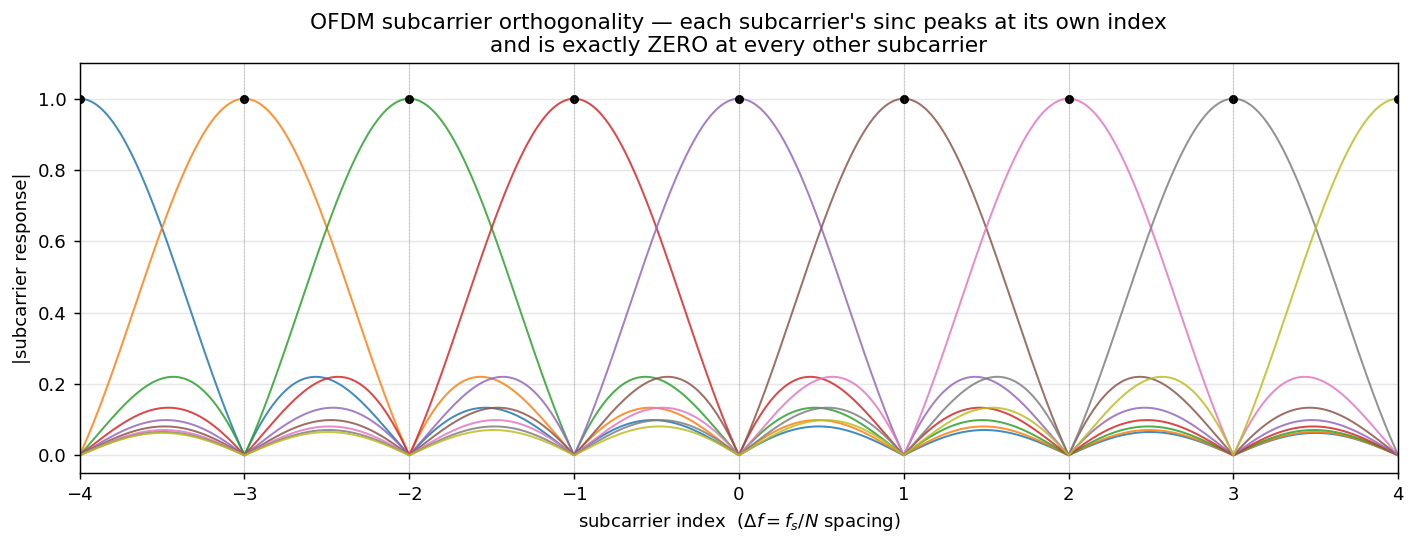
\includegraphics{figures/ofdm_orthogonality.png}

\textbf{Channel estimation \& pilots.} One known
\textbf{channel-estimation symbol} (known value on every active
subcarrier) gives \(H[k] = Y_\text{chest}[k]/\text{ref}[k]\).
\textbf{Scattered pilots} (every 8th active subcarrier carries a known
value) then track the residual \textbf{common phase error (CPE)} that
grows symbol-by-symbol from residual CFO.

\textbf{CPE estimation --- the fix that made OFDM work OTA.} Per data
symbol, estimate the phase φ from the pilots and derotate:

\[ \hat{\varphi} = \arg\!\Big( \sum_{k\,\in\,\text{pilots}} Y[k]\,H^{*}[k]\,\text{PILOT}^{*} \Big)
\qquad\text{(maximum-ratio combining)} \]

The earlier version used the \emph{equalized} pilot \(Y[k]/H[k]\), which
\textbf{blows up on a deep-fade subcarrier} (tiny
\textbar H{[}k{]}\textbar) --- one garbage pilot then hijacked φ and
smeared the whole symbol into a blob (EVM \textasciitilde67\%, 0 CRC
over the air; invisible in a mild simulation channel). Weighting by
channel power \texttt{\textbar{}H{[}k{]}\textbar{}\^{}2} via
\texttt{Y·conj(H)} suppresses faded pilots instead of amplifying them
-\textgreater{} four clean clusters (EVM \textasciitilde37\%), message
decodes. Disable with env \texttt{OFDM\_NO\_CPE=1} to compare.

\textbf{Common alternatives:} decision-feedback / per-subcarrier
phase-locked tracking, MMSE channel estimation (vs the least-squares one
used here), pilot-aided residual-CFO (SFO) slope correction,
windowed-OFDM / filtered-OFDM / OTFS for spectral containment.

\begin{center}\rule{0.5\linewidth}{0.5pt}\end{center}

\hypertarget{4-energy-detection-burst-gating}{%
\subsection{4. Energy detection (burst
gating)}\label{4-energy-detection-burst-gating}}

The RX runs continuously; the energy detector decides \emph{when a burst
is present} so downstream sync isn't run on noise.

\textbf{Math.} This is a \textbf{binary hypothesis test} per sample ---
\(H_0\): noise only, \(H_1\): signal present --- on the received power.
The instantaneous power \(|r[n]|^2\) is smoothed by a one-pole IIR
(exponential moving average) to reduce variance:

\[ P[n] = (1-\alpha)\,|r[n]|^2 + \alpha\,P[n-1], \qquad \text{declare burst if } P[n] > \gamma. \]

Larger \(\alpha\) = more averaging (time constant
\(\approx 1/(1-\alpha)\approx 20\) samples), which trades detection
latency for a lower false-alarm rate --- the smoothing collapses the
variance of the noise-power estimate so a single threshold \(\gamma\)
cleanly separates the two hypotheses. (\(\alpha=0.02\) barely smoothed
-\textgreater{} the detector fired on every noise spike and even chopped
real bursts apart on the RRC envelope; \(\alpha=0.95\) gives one clean
capture/burst.)

\begin{itemize}
\tightlist
\item
  \textbf{Adaptive threshold} (\texttt{-\/-det-adaptive\ true},
  default): \(\gamma = \nu \cdot \hat{N}_0\) where \(\hat{N}_0\) is the
  measured noise floor and \(\nu\) = \texttt{-\/-det-mult\ 5} (raise to
  10--30 over the air so ambient RF doesn't trigger it; too high misses
  weak bursts).
\item
  \textbf{Continuous noise tracking} (\texttt{-\/-det-continuous\ true},
  default): the noise floor itself is re-estimated by an EMA during idle
  periods,
  \(\hat{N}_0 \leftarrow (1-\beta)\hat{N}_0 + \beta\,|r[n]|^2\), so it
  follows drifting ambient noise. Alternative: one-shot startup
  calibration (\texttt{-\/-det-continuous\ false}) --- simpler but
  brittle if the environment changes.
\item
  \textbf{Fixed threshold} (\texttt{-\/-det-adaptive\ false} +
  \texttt{-\/-det-threshold\ 1e-7}): absolute cutoff, only for a known
  clean cabled link.
\item
  \texttt{-\/-energy\_packet\_size} --- how many samples to grab once a
  burst is detected (auto-sized per modulation).
\end{itemize}

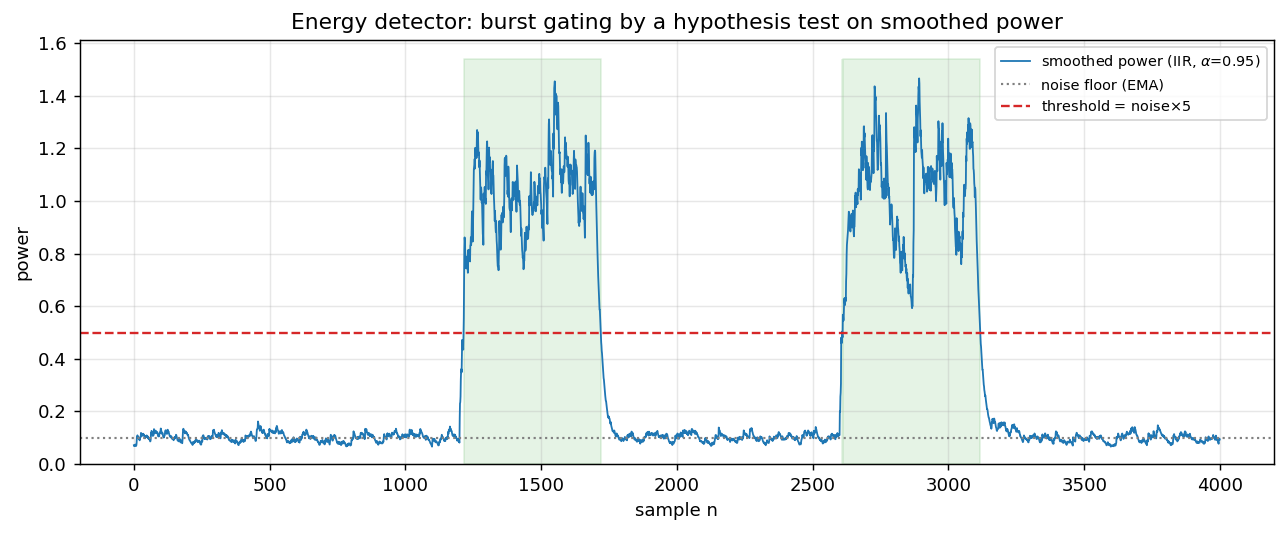
\includegraphics{figures/energy_detector.png}

\textbf{Common alternatives:} matched-filter / correlation detection
(detect on the \emph{known preamble} rather than energy --- more
sensitive but needs the template), constant-false-alarm-rate (CFAR)
detectors, cyclostationary feature detection (works below the noise
floor).

\begin{center}\rule{0.5\linewidth}{0.5pt}\end{center}

\hypertarget{5-synchronization-frequency--phase-offset}{%
\subsection{5. Synchronization, frequency \& phase
offset}\label{5-synchronization-frequency--phase-offset}}

\hypertarget{50-the-received-signal-model-what-every-block-below-is-undoing}{%
\subsubsection{5.0 The received-signal model (what every block below is
undoing)}\label{50-the-received-signal-model-what-every-block-below-is-undoing}}

After the RX front-end down-converts to baseband, the transmitted symbol
stream \texttt{s{[}m{]}} (pulse-shaped, sampled at \texttt{fs}) arrives
distorted by four separable impairments:

\[ r[n] = \underbrace{A\;e^{\,j\left(2\pi\frac{\Delta f}{f_s} n + \varphi_0\right)}}_{\text{carrier}}
\underbrace{\sum_m s[m]\,g\!\left(nT_s - mT - \tau\right)}_{\text{timing (delay }\tau)}
\;+\; \underbrace{w[n]}_{\text{noise}} \]

\begin{itemize}
\tightlist
\item
  \(A\) --- unknown gain -\textgreater{} removed by the \textbf{AGC}
  (§9).
\item
  \(\Delta f\) --- \textbf{carrier frequency offset (CFO)}: the two
  radios' oscillators differ (each B210 TCXO is ±2 ppm, so up to
  \textasciitilde4 ppm ≈ 3.6 kHz at 915 MHz). A constant \(\Delta f\)
  produces a phase that \textbf{grows linearly with time},
  \(\theta[n] = 2\pi(\Delta f/f_s)\,n\) --- it \emph{spins} the
  constellation. Left uncorrected it turns the constellation into a
  ring.
\item
  \(\varphi_0\) --- \textbf{static carrier phase offset}: the
  oscillators' phase difference at acquisition plus the channel's phase.
  A constant \emph{rotation} of the whole constellation.
\item
  \(\tau\) --- \textbf{timing offset}: the ADC sampling grid isn't
  aligned to the symbol centers, so the matched filter is sampled off
  its peak -\textgreater{} inter-symbol interference (ISI).
\item
  \(w[n]\) --- AWGN.
\end{itemize}

Note the coupling: \textbf{residual CFO becomes a phase ramp}
\(\varphi[n] = \varphi_0 + 2\pi(\Delta f/f_s)\,n\), which is why §5.5
uses a \emph{second-order} loop (tracks a constant phase \textbf{and}
its constant rate) and why OFDM needs per-symbol CPE tracking (§3.2).
The recovery order is: \textbf{frame sync -\textgreater{} timing
-\textgreater{} CFO -\textgreater{} phase}.

\hypertarget{51-preamble-the-known-reference-all-estimators-key-off}{%
\subsubsection{5.1 Preamble (the known reference all estimators key
off)}\label{51-preamble-the-known-reference-all-estimators-key-off}}

\texttt{-\/-preamble\ m-sequence} (default) or
\texttt{-\/-preamble\ zadoff}; \texttt{-\/-m\ 5} sets the m-sequence
order (length \texttt{L\ =\ 2\^{}m\ −\ 1\ =\ 31}).

A good preamble \(p\) has a \textbf{thumbtack autocorrelation}
\(\sum_n p[n]\,p^{*}[n+k] \approx E\,\delta[k]\) (large at zero lag,
near-zero elsewhere) so the correlator (§5.2) gives one sharp,
unambiguous peak.

\begin{itemize}
\tightlist
\item
  \textbf{m-sequence} --- maximal-length binary (BPSK ±1) shift-register
  sequence. Periodic autocorrelation is two-valued: \(L\) at zero lag,
  \(-1\) otherwise. Real-valued.
\item
  \textbf{Zadoff-Chu} --- complex \textbf{CAZAC} sequence
  \(p[n] = e^{-j\pi u\, n(n+1)/L}\): \emph{constant amplitude} and
  \emph{zero cyclic autocorrelation}. The flat spectrum makes it ideal
  for training a complex channel estimate / equalizer, and its constant
  envelope correlates cleanly even under CFO. Preferred for equalizer
  training and dense QAM.
\end{itemize}

For \textbf{differential} schemes the \textbf{last preamble symbol
doubles as the differential reference}: the TX encodes the first data
symbol relative to it, and the RX keeps that one symbol in front of the
data so the differential decoder returns exactly \(N\) symbols (not
\(N-1\)). This keeps the decoded bit count aligned with the fixed
FEC/CRC/ARQ framing, and these schemes bypass the coherent phase PLL
(§5.5) --- a decision-directed loop would pin the absolute phase and
destroy the transitions they carry. (The equalizer path prepends the
\emph{ideal} \texttt{preamble.back()} instead, since equalization has
already normalized the data to the ideal frame.) Hardware-verified
end-to-end for DBPSK / DQPSK / 8-DPSK; without this the reference
off-by-one shifted the framing and every packet failed even though sync
was perfect.

\hypertarget{52-frame-synchronization--acq-correlation}{%
\subsubsection{5.2 Frame synchronization --- ACQ
correlation}\label{52-frame-synchronization--acq-correlation}}

The receiver must find where the packet starts.
\texttt{ACQSynchronizer::SamplesACQPerformance} slides the known
preamble over the burst and computes, at each candidate offset τ (the
\texttt{ComputeCorrelation} routine), the \textbf{matched-filter /
cross-correlation} magnitude:

\[ R(\tau) = \left| \sum_{n=0}^{L-1} p^{*}[n]\; r[\,\tau + n\,o_s\,] \right|
\qquad (o_s = \text{samples/symbol}) \]

By the matched-filter theorem this is the optimal detector for a known
sequence in AWGN. At the true start \(\tau^{*}\), all \(L\) terms add
coherently -\textgreater{} \(R(\tau^{*}) \approx \sum|p[n]|^2\); at any
wrong offset the terms add with random phases -\textgreater{}
\(R \sim \sqrt{L}\) (much smaller). Detection:

\begin{itemize}
\tightlist
\item
  \textbf{Coarse pass}: find \(\tau\) where \(R(\tau)\) first crosses
  \texttt{-\/-sync\_threshold} (default 15), then
\item
  \textbf{Fine pass}: search ±a few samples around it for the true
  maximum.
\item
  \textbf{Noise floor / CFAR}: \texttt{EstimateNoiseFloor} correlates
  \emph{away} from the peak (excluding a guard zone) to measure the
  off-peak floor, so the threshold can be set relative to it. Set
  \texttt{-\/-sync-threshold} below the real peak (≈ preamble length
  \textasciitilde31 after AGC) but above that floor; watch the
  \texttt{{[}ACQ{]}\ Peak\ correlation} log lines.
\end{itemize}

Because the search tests \textbf{every sample} (not every
\texttt{os}-th), the peak location simultaneously gives \textbf{coarse
symbol timing} --- the correct sub-symbol sampling phase. (Striding by
\texttt{os} would test only one of the \texttt{os} phases and could lock
a half-symbol off -\textgreater{} catastrophic ISI, BER ≈ 0.5. This was
an actual bug; the brute-force search fixed it.)

\hypertarget{53-symbol-timing-recovery--acq-active-vs-gardner-ted-available}{%
\subsubsection{5.3 Symbol-timing recovery --- ACQ (active) vs Gardner
TED
(available)}\label{53-symbol-timing-recovery--acq-active-vs-gardner-ted-available}}

\textbf{What actually runs: ACQ, not Gardner.} In packet mode the symbol
timing is recovered \emph{entirely} by the ACQ preamble correlation of
§5.2 --- because the correlator tests \textbf{every} sample offset, its
peak already lands on the optimal sub-symbol sampling instant, and the
aligned burst is extracted at one sample/symbol. No separate timing loop
runs. This is a \textbf{feedforward, one-shot per-burst} estimate: fast,
robust, and sufficient here because the sample-clock (SFO) drift across
a single \textasciitilde1000-symbol burst is negligible (≈ 0.004 symbols
at 4 ppm), so one timing phase holds for the whole burst.

\textbf{Available but dormant: the Gardner timing-error detector.}
\texttt{GardnerTED} and a ready \texttt{timing\_recovery\_thread} live
in \texttt{timing\_recovery.hpp}, and its knobs are exposed
(\texttt{-\/-timing\_loop\_bw\ 0.015},
\texttt{-\/-timing\_damping\ 0.707}), but it is \textbf{not wired into
the current RX pipeline} --- ACQ replaced it, and those two parameters
are currently unconsumed (Gardner is exercised only by
\texttt{tests/frontend\_repro.cpp}). It is a \emph{feedback} loop that
tracks a continuously \textbf{drifting} fractional delay, which is
needed only for a \textbf{true continuous symbol stream} (no per-burst
preamble to re-sync on), where SFO accumulates over millions of symbols
into whole-symbol drift. Drop it in between the matched filter and the
CFO stage if/when such a waveform is added. The rest of this section
describes that (available) detector.

\textbf{Error detector.} With two samples per symbol --- one at the
symbol center \(y_k\) and one at the half-symbol midpoint \(y_{k-1/2}\)
--- the Gardner error is

\[ e_k = \mathrm{Re}\!\left\{\, (y_k - y_{k-1})\; y_{k-1/2}^{*} \,\right\}. \]

Intuition: if sampling is early or late, the midpoint sample
\(y_{k-1/2}\) (sitting on the transition between symbols) correlates
with the slope \(y_k - y_{k-1}\); at perfect timing the midpoint is a
true zero-crossing and \(e_k = 0\). It is \textbf{decision-independent
and carrier-phase-independent} (the \(\mathrm{Re}\{\cdot\}\) with the
difference term cancels a constant rotation), so it works \emph{before}
CFO/phase are resolved --- the classic reason Gardner is favoured for
QAM \emph{tracking} loops.

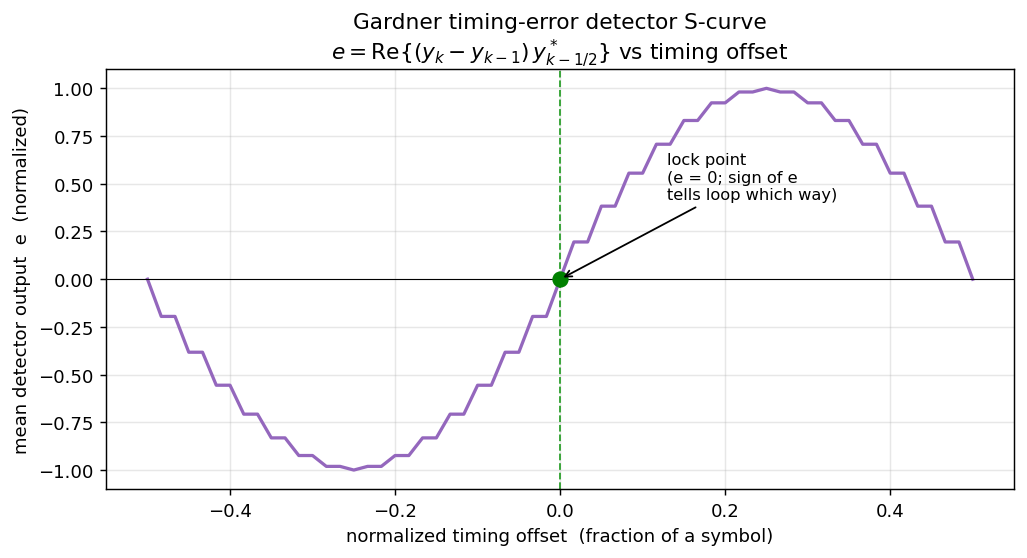
\includegraphics{figures/gardner_scurve.png}

\textbf{Loop.} The NCO advances \(\omega = 2/\text{sps}\) per input
sample (two strobes/symbol --- using \(1/\text{sps}\) gives only one
strobe and the "midpoint" lands a full symbol away -\textgreater{} the
loop tracks garbage; this was a fixed bug). A \textbf{Farrow
interpolator} produces the fractional-delay sample at offset \(\mu\),
and a \textbf{proportional-integral (PI) loop filter} drives \(\mu\):

\[ \nu \mathrel{+}= K_2\, e_k \quad(\text{integrator — tracks a constant timing rate / clock offset}),
\qquad \mu \mathrel{-}= K_1\, e_k \quad(\text{proportional}). \]

with \(\nu\) clamped to ±10 \% of \(\omega\). The PI coefficients come
from the standard second-order design (same \(\theta_n\)/\(\zeta\)
formulas as §5.5). Only the symbol-center strobes are emitted
-\textgreater{} exactly one sample per symbol out.

\emph{Alternatives:} Mueller \& Müller (decision-directed, needs only 1
sample/sym but needs carrier first), early-late gate, zero-crossing TED.

\hypertarget{54-carrier-frequency-offset-cfo-estimation--correction}{%
\subsubsection{5.4 Carrier frequency offset (CFO) estimation \&
correction}\label{54-carrier-frequency-offset-cfo-estimation--correction}}

A constant CFO spins the constellation at \(2\pi\,\Delta f/f_s\)
rad/sample. Two estimators are provided (\texttt{CFOEstimator}), both
\textbf{data-aided} off the preamble, then \texttt{FrequencyShifter}
removes it by multiplying sample \(n\) by \(e^{-j2\pi(\Delta f/f_s)n}\)
(a running phase accumulator, so blocks join seamlessly).

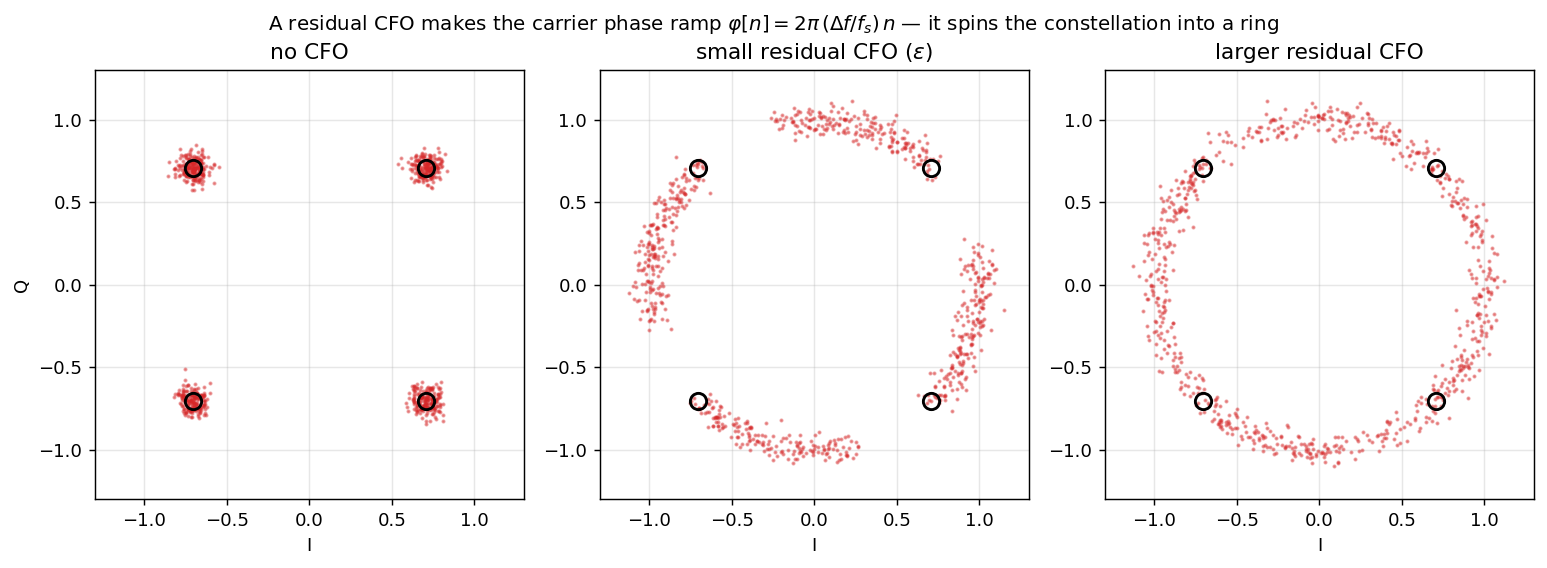
\includegraphics{figures/cfo_effect.png}

\textbf{(A) Pilot-aided (phase-slope across preamble symbols).} For
preamble symbols \(p[k]\) received at \(r[k\cdot\text{sps}]\), the phase
advance per symbol is measured with the known data stripped off:

\[ \varphi_k = \arg\!\big(\, r[k\,\text{sps}]\; r^{*}[(k{-}1)\text{sps}]\; p^{*}[k]\; p[k{-}1] \,\big),
\qquad \widehat{\Delta f} = \frac{f_s}{2\pi\,\text{sps}}\;\overline{\varphi_k}. \]

Averaging over the preamble reduces noise. Unambiguous range
\(|\Delta f| < f_s/(2\,\text{sps})\) (one symbol of phase must not
wrap).

\textbf{(B) Auto-correlation (Moose / Schmidl-Cox).} With a preamble
made of two identical halves of length \(L\), the second half equals the
first times the CFO phase accrued over \(L\) samples:

\[ P = \sum_{n=0}^{L-1} r[n]\; r^{*}[n+L] \;\approx\; |A|^2 L\; e^{\,j2\pi(\Delta f/f_s)L},
\qquad \widehat{\Delta f} = \frac{f_s}{2\pi L}\,\arg(P). \]

Unambiguous range \(|\Delta f| < f_s/(2L)\) --- smaller \(L\)
-\textgreater{} wider capture range but noisier. This is the same
estimator OFDM uses (§5.6), where \(L = N/2\).

\textbf{Why residual CFO still matters.} \(\arg(\cdot)\) limits the
estimate; whatever is left is a slow phase ramp the \textbf{phase
tracker (§5.5)} or \textbf{OFDM pilot CPE (§3.2)} cleans up. Getting
this balance wrong is exactly what smeared 16-QAM/OFDM over the air.

\hypertarget{55-carrier-phase-offset--estimation--pll-tracking}{%
\subsubsection{5.5 Carrier phase offset --- estimation \& PLL
tracking}\label{55-carrier-phase-offset--estimation--pll-tracking}}

After timing + CFO the symbols still carry a residual phase
\(\varphi[n] = \varphi_0 + (\text{residual ramp})\). For
\textbf{absolute} constellations (BPSK/QPSK/QAM) all of it must be
removed before hard decisions; for \textbf{differential} schemes the
static \(\varphi_0\) cancels automatically (demod uses phase
\emph{differences}).

\textbf{One-shot estimators} (\texttt{PhaseOffsetEstimator}):

\begin{itemize}
\tightlist
\item
  \textbf{ML / preamble correlation} --- optimal given the known
  preamble: \(\hat{\varphi} = \arg\!\big(\sum_n r[n]\,p^{*}[n]\big)\).
\item
  \textbf{M-th power (blind, for M-PSK)} --- raising to the \(M\)-th
  power collapses all \(M\) data phases onto one, removing the
  modulation:
  \(\hat{\varphi} = \tfrac{1}{M}\arg\!\big(\sum_n r[n]^{M}\big)\).
\item
  \textbf{Decision-directed} ---
  \(\hat{\varphi} = \arg\!\big(\sum_n r[n]\,\hat{s}^{*}[n]\big)\)
  against the nearest constellation points \(\hat{s}\) (used for QAM,
  after a coarse lock).
\end{itemize}

\textbf{Tracking PLL} (\texttt{PhaseTracker}) --- a second-order digital
PLL that follows a static offset \textbf{and} a constant frequency ramp
(residual CFO). Per symbol: form the phase error against the nearest
decision, then update an integrator (frequency) and the phase:

\[
\begin{aligned}
e[n] &= \arg\!\big(\, \text{corrected}[n]\;\hat{s}^{*}[n] \,\big) &&\text{(phase detector, angle in }[-\pi,\pi]) \\
\text{freq} &\mathrel{+}= \beta\, e[n] &&\text{(integrator — tracks the residual CFO ramp)} \\
\varphi &\mathrel{+}= \alpha\, e[n] + \text{freq} &&\text{(NCO phase)}
\end{aligned}
\]

The loop coefficients come from the standard proportional-integral
design for loop bandwidth \(B_n T\) (\texttt{-\/-phase\_loop\_bw\ 0.02})
and damping \(\zeta\) (\texttt{-\/-phase\_damping\ 0.707}):

\[ \theta_n = \frac{B_n T}{\zeta + 1/(4\zeta)}, \qquad
\alpha = \frac{4\zeta\,\theta_n}{1 + 2\zeta\,\theta_n + \theta_n^{2}}, \qquad
\beta  = \frac{4\,\theta_n^{2}}{1 + 2\zeta\,\theta_n + \theta_n^{2}}. \]

(\(\beta = 0\) gives a first-order loop.) Smaller \(B_n T\) = less
jitter but slower pull-in; \(\zeta = 0.707\) is the critically-damped
standard.

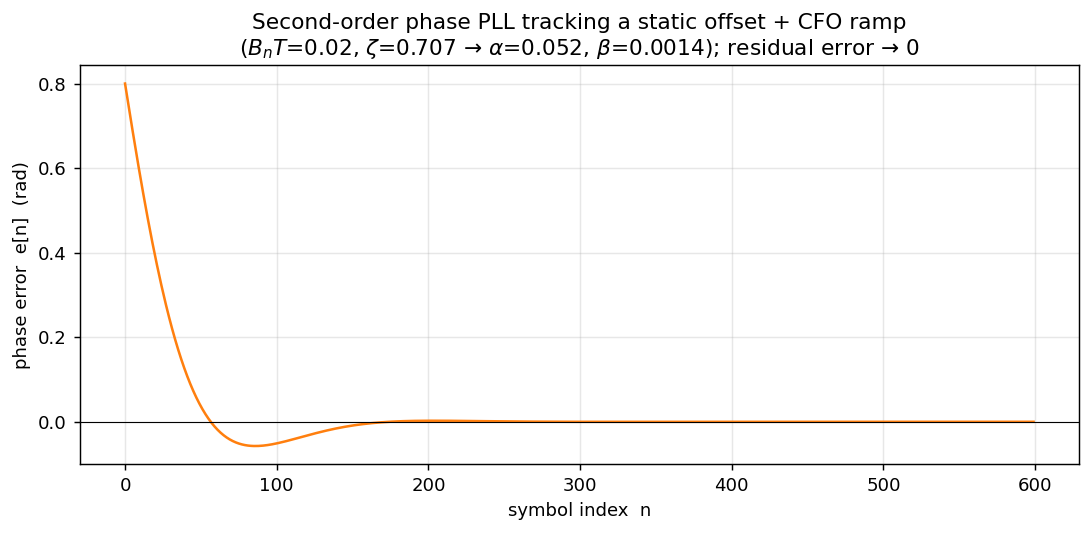
\includegraphics{figures/pll_convergence.png}

\emph{Alternatives:} Costas loop (joint carrier recovery on the raw
samples), block Viterbi-Viterbi phase estimation, pilot-symbol-aided
interpolation.

\hypertarget{56-ofdm-synchronization--schmidl--cox}{%
\subsubsection{5.6 OFDM synchronization --- Schmidl \&
Cox}\label{56-ofdm-synchronization--schmidl--cox}}

OFDM recovers frame timing and CFO jointly from a sync symbol built as
two identical time halves \texttt{{[}A\ A{]}} (generated by loading only
the \textbf{even} subcarriers). Sliding a window of length \texttt{N/2}:

\[
\begin{aligned}
P(d) &= \sum_{n=0}^{N/2-1} r[d+n]\; r^{*}[d+n+N/2] &&\text{(half-to-half correlation)} \\
R(d) &= \sum_{n=0}^{N/2-1} \big|\,r[d+n+N/2]\,\big|^{2} &&\text{(energy normaliser)} \\
M(d) &= |P(d)|^{2} / R(d)^{2} &&\text{(timing metric} \in [0,1])
\end{aligned}
\]

\(M(d)\) forms a \textbf{plateau} where the two halves align; the frame
start is the plateau's left edge plus a small guard into the CP (any
offset inside the CP is just a per-subcarrier phase the channel estimate
absorbs). The \textbf{fractional CFO} falls out of the same correlation:

\[ \hat{\epsilon} = \arg(P)\,/\,\pi \qquad \text{(subcarrier-spacing units, range } \pm 1 \text{ subcarrier)}. \]

and the burst is derotated by \(e^{-j2\pi\epsilon n/N}\). Residual CFO /
phase drift across the frame is then tracked per symbol by the
scattered-pilot CPE of §3.2. An energy gate (\(R \ge 0.30\,\max R\))
stops the metric from locking onto the low-power noise pad before the
burst.

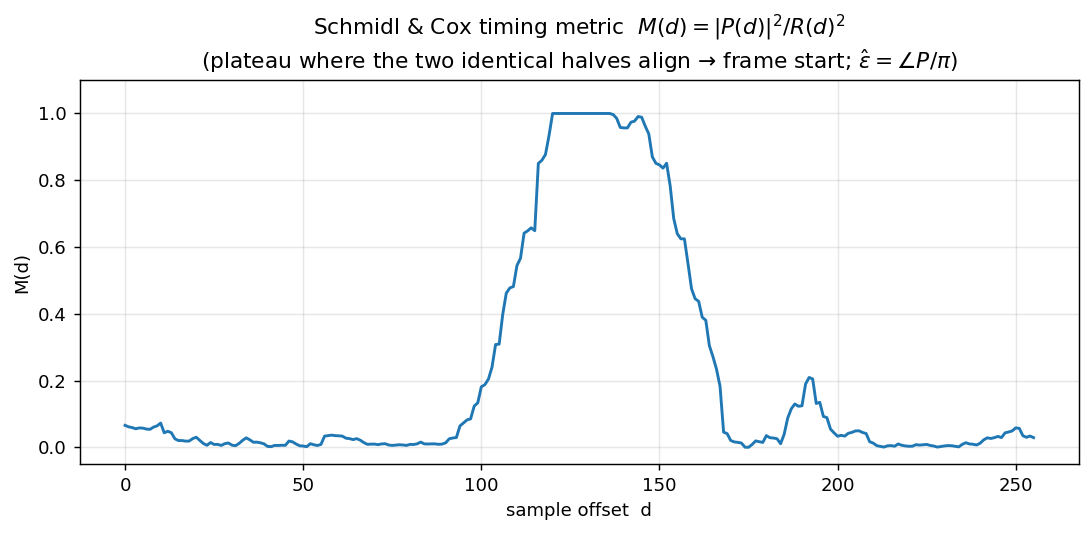
\includegraphics{figures/schmidl_cox.png}

\emph{Alternatives:} Minn and Park metrics (sharper, no plateau
ambiguity), CP-based blind sync.

\begin{center}\rule{0.5\linewidth}{0.5pt}\end{center}

\hypertarget{6-channel-equalization-single-carrier}{%
\subsection{6. Channel equalization
(single-carrier)}\label{6-channel-equalization-single-carrier}}

\texttt{-\/-eq\_type\ None} (default) \textbar{} \texttt{LMS} \textbar{}
\texttt{RLS} \textbar{} \texttt{DFE}. \texttt{-\/-eq\_taps\ 11},
\texttt{-\/-eq\_mu\ 0.3} (NLMS step), \texttt{-\/-eq\_dd\ false}
(decision-directed tracking after training).

\textbf{Math.} A length-\(T\) linear FIR equalizer \(w\) estimates each
symbol from a window of received samples,
\(\hat{s}[k] = w^{H} r[k] = \sum_i w_i^{*}\, r[k-i]\), choosing \(w\) to
invert the channel \(h\) (ideally \(w * h \approx \delta\)). Two ways to
find \(w\):

\begin{itemize}
\item
  \textbf{Least-squares / MMSE training} (used, exact for the complex
  Zadoff-Chu preamble). Stack the preamble windows into a matrix \(R\)
  and the known symbols into \(s\); minimizing
  \(\lVert Rw - s \rVert^{2}\) gives the normal equations

  \[ w = \big(R^{H} R + \lambda I\big)^{-1} R^{H} s \]

  solved here by Gaussian elimination. \(\lambda I\) = Tikhonov /
  diagonal-loading regularization: it bounds noise enhancement at
  channel nulls (the MMSE, not zero-forcing, solution).
\item
  \textbf{NLMS adaptive update} (real preamble / decision-directed
  tracking): step down the instantaneous-error gradient, normalized by
  input power for stability:

  \[ e[k] = s[k] - \hat{s}[k], \qquad
  w \leftarrow w + \mu\,\frac{e^{*}[k]\, r[k]}{\lVert r[k]\rVert^{2} + \varepsilon}
  \quad(\texttt{--eq\_mu}\ 0.3,\; 0 < \mu < 2). \]
\end{itemize}

The LS solution places the main tap at the equalizer center, so a
\textbf{center-tap group delay} of \((T-1)/2\) samples must be
compensated when aligning the output --- mishandling this looked like
"divergence" and was a fixed bug.

\textbf{Status / why default None.} On a clean cabled link no equalizer
is needed. The LMS decision-directed loop currently \textbf{diverges on
the real hardware signal} (DD error grows and destroys the symbols) ---
verified OTA where \texttt{None} decodes and \texttt{LMS} produces
garbage. For frequency-selective channels, prefer \textbf{OFDM} (§3.2),
which equalizes per-subcarrier without an adaptive FIR. Alternatives:
DFE (feedback of past decisions, better on deep nulls), RLS (faster
convergence than LMS, O(n\^{}2) cost), MLSE/Viterbi equalization
(optimal, expensive).

\begin{center}\rule{0.5\linewidth}{0.5pt}\end{center}

\hypertarget{7-forward-error-correction-fec}{%
\subsection{7. Forward error correction
(FEC)}\label{7-forward-error-correction-fec}}

\texttt{-\/-fec\ true} (default off) --- rate-1/2, constraint-length-7
\textbf{convolutional code} with \textbf{Viterbi} hard-decision
decoding. Must match on both ends; halves the payload rate (2× symbols).

\textbf{Math.} Encoder: a 6-stage shift register holds the last
\(K-1 = 6\) input bits (state \(\sigma \in \{0,\dots,63\}\)); each input
bit \(u\) emits two coded bits as mod-2 (XOR) taps of the register per
the generator polynomials \(G_1 = 171_8\), \(G_2 = 133_8\) (the standard
NASA / 802.11a code):

\[ c_1 = G_1 \cdot [u,\sigma] \bmod 2, \qquad c_2 = G_2 \cdot [u,\sigma] \bmod 2. \]

Each input bit thus influences \(K = 7\) output-bit pairs (the
constraint length / memory), which is what lets the decoder recover it
even when some of those bits are flipped.

\textbf{Viterbi decoding} finds the maximum-likelihood transmitted
sequence by the most-likely path through the 64-state trellis. For hard
decisions the branch metric is the \textbf{Hamming distance} between the
received pair and each branch's expected \((c_1,c_2)\); the decoder
keeps, per state, the survivor path with the smallest cumulative metric:

\[ \text{PM}_t(\sigma') = \min_{\sigma \,\to\, \sigma'}
\Big[\, \text{PM}_{t-1}(\sigma) + d_H\big(r_t,\; c(\sigma\!\to\!\sigma')\big) \,\Big] \]

then traces the survivors back to output the bits. It corrects any error
pattern up to roughly \(\lfloor (d_\text{free}-1)/2 \rfloor\) ---
\(d_\text{free} = 10\) for this code --- per window; validated
\textasciitilde100 \% CRC-OK up to \textasciitilde2 \% raw BER. (Two
original bugs --- encoder emitting from the \emph{next} state, traceback
storing the bit instead of the predecessor state --- were fixed.)
\textbf{Soft-decision} Viterbi (Euclidean instead of Hamming metric,
using the raw symbol distances) would add \textasciitilde2 dB but isn't
implemented.

\textbf{Common alternatives:} LDPC and Turbo codes (near-Shannon, used
in Wi-Fi/5G), Reed-Solomon (burst errors), Polar codes (5G control),
soft-decision Viterbi (\textasciitilde2 dB better than the hard-decision
decoder here).

\begin{center}\rule{0.5\linewidth}{0.5pt}\end{center}

\hypertarget{8-error-detection--arq}{%
\subsection{8. Error detection + ARQ}\label{8-error-detection--arq}}

\begin{itemize}
\tightlist
\item
  \textbf{CRC-16-CCITT} appended to every chunk; the RX drops any chunk
  that fails the check (guarantees the delivered message is error-free).
\item
  \textbf{Stop-and-wait ARQ} (\texttt{-\/-role\ source\_arq} /
  \texttt{sink\_arq}): the source sends a chunk and waits for an ACK; on
  \texttt{-\/-timeout\ 3000} ms it retransmits; it advances when ACKed
  and exits when all chunks are ACKed. The sink CRC-verifies each chunk,
  ACKs only verified ones, re-ACKs duplicates, and auto-stops once every
  chunk is in.
\item
  \textbf{ACK transport} (\texttt{-\/-ack-transport}):

  \begin{itemize}
  \tightlist
  \item
    \texttt{tcp} (default) --- ACK over a socket; \textbf{no reverse RF
    path needed}. Source connects to
    \texttt{-\/-ack-host\ 127.0.0.1\ :\ -\/-ack-port\ 5599} (the sink
    listens there). Ideal when both radios share one host.
  \item
    \texttt{rf} --- ACK sent back over the air on the second RF path
    (needs a clean reverse link).
  \end{itemize}
\end{itemize}

\textbf{Math/theory.} Treat the message bits as coefficients of a
polynomial \(M(x)\) over GF(2); append 16 zeros (\(M(x)\cdot x^{16}\))
and divide by the CRC-16-CCITT generator
\(G(x) = x^{16}+x^{12}+x^{5}+1\) (mod-2 / XOR long division). The 16-bit
remainder is the CRC; the RX recomputes it and flags any nonzero
mismatch. Because an undetected error requires the error polynomial
\(E(x)\) to be an exact multiple of \(G(x)\), this structure guarantees
detection of: all single- and double-bit errors, any odd number of
errors (\(G\) has the factor \(x+1\)), and all burst errors of length
\(\le 16\). Residual undetected probability \(\approx 2^{-16}\) for
random errors.

Stop-and-wait is the simplest ARQ (throughput limited by idling one
round-trip per chunk). \emph{Alternatives:} Go-Back-N / Selective-Repeat
(pipelined, higher throughput), Hybrid-ARQ (FEC + ARQ combined --- what
you get here with \texttt{-\/-fec} on: FEC corrects most errors,
CRC+retransmit catches the rest).

\textbf{One-way mode} (\texttt{-\/-role\ tx} / \texttt{rx}, no ACK): the
TX cycles all chunks \texttt{-\/-tx-reps} times; the RX reassembles from
CRC-verified chunks and auto-stops \texttt{-\/-rx-idle-timeout\ 8} s
after the last burst.

\begin{center}\rule{0.5\linewidth}{0.5pt}\end{center}

\hypertarget{9-automatic-gain-control-agc}{%
\subsection{9. Automatic gain control
(AGC)}\label{9-automatic-gain-control-agc}}

\texttt{-\/-AGC\_type\ Feed} (feed-forward, default) or \texttt{Closed}
(closed-loop). Feed-forward measures the detected burst's RMS and scales
it to unit power in one shot (no loop lag); closed-loop adapts a gain
over time. The energy detector's captured burst feeds the AGC before
sync.

\begin{center}\rule{0.5\linewidth}{0.5pt}\end{center}

\hypertarget{10-visualization--evm}{%
\subsection{10. Visualization / EVM}\label{10-visualization--evm}}

\texttt{-\/-viz\ true} (default) captures one TX and one RX burst and
\textbf{auto-saves a figure on exit} to
\texttt{\textless{}viz-dir\textgreater{}/\textless{}scheme\textgreater{}/figure.png}
(per-modulation folder, \texttt{-\/-viz-dir\ viz}). The 2×3 figure shows
TX/RX \textbf{time domain}, \textbf{spectrum} (FFT), and
\textbf{constellation} with the ideal points overlaid and an \textbf{EVM
\%} readout. Rough EVM ceilings for reliable decode: QPSK tolerates
\textasciitilde30--35\% (more with FEC), 16-QAM needs
\textless\textasciitilde12\%, 64-QAM \textless\textasciitilde6\%. Render
manually with
\texttt{python3\ tools/plot\_viz.py\ \textless{}dir\textgreater{}\ -\/-fs\ 1.6e6\ -\/-save\ out.png}.

\begin{center}\rule{0.5\linewidth}{0.5pt}\end{center}

\hypertarget{11-complete-command-line-reference}{%
\subsection{11. Complete command-line
reference}\label{11-complete-command-line-reference}}

\hypertarget{mode--roles}{%
\subsubsection{Mode / roles}\label{mode--roles}}

\begin{longtable}[]{@{}lll@{}}
\toprule
Option & Default & Controls \\
\midrule
\endhead
\texttt{-\/-role} & \texttt{both} & \texttt{tx}, \texttt{rx},
\texttt{both}, \texttt{source\_arq}, \texttt{sink\_arq} \\
\texttt{-\/-mode} & \texttt{source} & legacy source/sink selector \\
\texttt{-\/-tx-reps} & \texttt{20} & one-way: times to cycle all chunks
(no ACK) \\
\texttt{-\/-rx-idle-timeout} & \texttt{8.0} & one-way RX: auto-stop
after N s of no bursts (0 = until Ctrl-C) \\
\texttt{-\/-num\_bits} & \texttt{1000} & payload bits per packet \\
\texttt{-\/-interval} & \texttt{3000} & TX gap between packets (ms) \\
\bottomrule
\end{longtable}

\hypertarget{arq--ack}{%
\subsubsection{ARQ / ACK}\label{arq--ack}}

\begin{longtable}[]{@{}lll@{}}
\toprule
Option & Default & Controls \\
\midrule
\endhead
\texttt{-\/-ack-transport} & \texttt{tcp} & ACK channel: \texttt{tcp} or
\texttt{rf} \\
\texttt{-\/-ack-host} & \texttt{127.0.0.1} & TCP: sink IP the source
connects to \\
\texttt{-\/-ack-port} & \texttt{5599} & TCP: ACK socket port \\
\texttt{-\/-timeout} & \texttt{3000} & source ACK timeout (ms) before
retransmit \\
\texttt{-\/-timer\_interval} & \texttt{1000} & sink ACK timer interval
(ms) \\
\bottomrule
\end{longtable}

\hypertarget{modulation--waveform--fec}{%
\subsubsection{Modulation / waveform /
FEC}\label{modulation--waveform--fec}}

\begin{longtable}[]{@{}lll@{}}
\toprule
Option & Default & Controls \\
\midrule
\endhead
\texttt{-\/-scheme} & \texttt{QPSK} & constellation (§2) \\
\texttt{-\/-fec} & \texttt{false} & rate-1/2 K=7 conv + Viterbi (must
match both ends) \\
\texttt{-\/-waveform} & \texttt{sc} & \texttt{sc} (single-carrier) or
\texttt{ofdm} \\
\texttt{-\/-ofdm-fft} & \texttt{64} & OFDM subcarrier count (FFT
size) \\
\texttt{-\/-ofdm-cp} & \texttt{16} & OFDM cyclic-prefix length \\
\texttt{-\/-ofdm-tx-peak} & \texttt{0.5} & OFDM peak scaling (PAPR /
clipping guard) \\
\texttt{-\/-sps} & \texttt{2} & samples/symbol (informational) \\
\bottomrule
\end{longtable}

\hypertarget{preamble--pulse-shaping}{%
\subsubsection{Preamble / pulse shaping}\label{preamble--pulse-shaping}}

\begin{longtable}[]{@{}lll@{}}
\toprule
Option & Default & Controls \\
\midrule
\endhead
\texttt{-\/-preamble} & \texttt{m-sequence} & \texttt{m-sequence} or
\texttt{zadoff} \\
\texttt{-\/-m} & \texttt{5} & m-sequence order (length 2\^{}m−1) \\
\texttt{-\/-add\_preamble} & \texttt{true} & prepend preamble to each
packet \\
\texttt{-\/-filter\_type} & \texttt{rrc} & \texttt{rrc} / \texttt{rc} /
\texttt{lp} \\
\texttt{-\/-roll\_off} & \texttt{0.25} & RRC/RC roll-off β \\
\texttt{-\/-num\_taps} & \texttt{151} & filter tap count \\
\texttt{-\/-U} / \texttt{-\/-D} & \texttt{2} / \texttt{1} & pulse-shaper
up/down sampling (wire sps = U/D) \\
\texttt{-\/-symbol\_rate} & \texttt{0.8e6} & symbol rate (Hz) \\
\texttt{-\/-num\_threads} & \texttt{1} & FFT threads \\
\bottomrule
\end{longtable}

\hypertarget{energy-detection}{%
\subsubsection{Energy detection}\label{energy-detection}}

\begin{longtable}[]{@{}lll@{}}
\toprule
Option & Default & Controls \\
\midrule
\endhead
\texttt{-\/-alpha} & \texttt{0.95} & IIR power-smoothing (larger =
smoother) \\
\texttt{-\/-det-adaptive} (\texttt{-\/-IIR\_threshold\_adaptive}) &
\texttt{true} & use noise\_floor×mult vs fixed threshold \\
\texttt{-\/-det-mult} (\texttt{-\/-IIR\_threshold\_multiplier}) &
\texttt{5.0} & adaptive threshold multiplier (raise OTA to 10--30) \\
\texttt{-\/-det-threshold} (\texttt{-\/-energy\_threshold}) &
\texttt{1e-7} & fixed threshold (adaptive off only) \\
\texttt{-\/-det-continuous} & \texttt{true} & re-track noise floor
during idle vs one-shot calib \\
\texttt{-\/-energy\_packet\_size} & \texttt{3300} & samples to collect
after detection (auto-sized) \\
\texttt{-\/-IIR\_window\_size} & \texttt{20} & IIR window size \\
\bottomrule
\end{longtable}

\hypertarget{synchronization--timing--phase}{%
\subsubsection{Synchronization / timing /
phase}\label{synchronization--timing--phase}}

\begin{longtable}[]{@{}lll@{}}
\toprule
Option & Default & Controls \\
\midrule
\endhead
\texttt{-\/-sync-threshold} (\texttt{-\/-sync\_threshold}) &
\texttt{15.0} & ACQ correlation gate (set below true peak, above
noise) \\
\texttt{-\/-sps\_sync} & \texttt{5} & samples/symbol at matched-filter
output \\
\texttt{-\/-recv\_msg\_len} & auto & data symbols to extract per burst
(auto from scheme) \\
\texttt{-\/-timing\_loop\_bw} & \texttt{0.015} & Gardner TED loop
bandwidth BnT \\
\texttt{-\/-timing\_damping} & \texttt{0.707} & Gardner TED damping \\
\texttt{-\/-phase\_loop\_bw} & \texttt{0.02} & carrier phase PLL
bandwidth \\
\texttt{-\/-phase\_damping} & \texttt{0.707} & carrier phase PLL
damping \\
\bottomrule
\end{longtable}

\hypertarget{equalizer}{%
\subsubsection{Equalizer}\label{equalizer}}

\begin{longtable}[]{@{}lll@{}}
\toprule
Option & Default & Controls \\
\midrule
\endhead
\texttt{-\/-eq\_type} & \texttt{None} & \texttt{None} / \texttt{LMS} /
\texttt{RLS} / \texttt{DFE} (see §6 --- LMS diverges OTA) \\
\texttt{-\/-eq\_taps} & \texttt{11} & equalizer tap count \\
\texttt{-\/-eq\_mu} & \texttt{0.3} & NLMS step (DD / real-preamble
training) \\
\texttt{-\/-eq\_dd} & \texttt{false} & decision-directed tracking after
LS training \\
\bottomrule
\end{longtable}

\hypertarget{rf-hardware-tx}{%
\subsubsection{RF hardware (TX)}\label{rf-hardware-tx}}

\begin{longtable}[]{@{}lll@{}}
\toprule
Option & Default & Controls \\
\midrule
\endhead
\texttt{-\/-tx-args} & \texttt{""} & UHD TX device (e.g.
\texttt{serial=30CD424}) \\
\texttt{-\/-tx-rate} & \texttt{1.6e6} & TX sample rate (Hz) =
symbol\_rate·U/D \\
\texttt{-\/-tx-freq} & \texttt{2.412e9} & TX centre frequency (Hz) \\
\texttt{-\/-tx-gain} & \texttt{20} & TX gain (dB) \\
\texttt{-\/-tx-bw} & \texttt{1.0e6} & TX analog bandwidth (Hz) \\
\texttt{-\/-tx-ant} & \texttt{TX/RX} & TX antenna port \\
\texttt{-\/-tx-subdev} & \texttt{A:A} & TX subdev spec \\
\texttt{-\/-tx-channel} & \texttt{0} & TX channel index \\
\bottomrule
\end{longtable}

\hypertarget{rf-hardware-rx}{%
\subsubsection{RF hardware (RX)}\label{rf-hardware-rx}}

\begin{longtable}[]{@{}lll@{}}
\toprule
Option & Default & Controls \\
\midrule
\endhead
\texttt{-\/-rx-args} & \texttt{""} & UHD RX device (e.g.
\texttt{serial=30CD3F7}) \\
\texttt{-\/-rx-rate} & \texttt{1.6e6} & RX sample rate (Hz), must equal
TX rate \\
\texttt{-\/-rx-freq} & \texttt{2.412e9} & RX centre frequency (Hz) \\
\texttt{-\/-rx-gain} & \texttt{30} & RX gain (dB) --- key for
EVM/clipping (§ recipes) \\
\texttt{-\/-rx-bw} & \texttt{1.0e6} & RX analog bandwidth (Hz) \\
\texttt{-\/-rx-ant} & \texttt{RX2} & RX antenna port \\
\texttt{-\/-rx-subdev} & \texttt{A:A} & RX subdev spec \\
\texttt{-\/-rx-channel} & \texttt{0} & RX channel index \\
\bottomrule
\end{longtable}

\hypertarget{common-rf--buffering--misc}{%
\subsubsection{Common RF / buffering /
misc}\label{common-rf--buffering--misc}}

\begin{longtable}[]{@{}lll@{}}
\toprule
Option & Default & Controls \\
\midrule
\endhead
\texttt{-\/-ref} & \texttt{internal} & clock reference:
\texttt{internal} / \texttt{external} / \texttt{mimo} \\
\texttt{-\/-settling} & \texttt{0.2} & RF settling time (s) \\
\texttt{-\/-uhd\_timeout} & \texttt{1000} & UHD TX timeout (ms) \\
\texttt{-\/-samps\_per\_buff} & \texttt{10000} & samples per UHD receive
buffer \\
\texttt{-\/-num\_recv\_request} & \texttt{0} & total samples to receive
(0 = continuous) \\
\texttt{-\/-AGC\_type} & \texttt{Feed} & \texttt{Feed} (feed-forward) or
\texttt{Closed} (closed-loop) \\
\texttt{-\/-dc-block} & \texttt{false} & experimental RX DC-block
high-pass (see §13) \\
\texttt{-\/-tx-dc-i} / \texttt{-\/-tx-dc-q} & \texttt{0} / \texttt{0} &
manual TX LO-leakage null, normalized {[}−1,1{]} (§13) \\
\texttt{-\/-skip-rate-check} & off & bypass startup rate-consistency
check \\
\texttt{-\/-viz} & \texttt{true} & capture + auto-save TX/RX figure on
exit \\
\texttt{-\/-viz-dir} & \texttt{viz} & base dir for figures (per-scheme
subfolder made) \\
\bottomrule
\end{longtable}

\begin{center}\rule{0.5\linewidth}{0.5pt}\end{center}

\hypertarget{12-command-reference--per-scheme-915-mhz-vert900-antennas}{%
\subsection{12. Command reference --- per scheme (915 MHz, VERT900
antennas)}\label{12-command-reference--per-scheme-915-mhz-vert900-antennas}}

Copy-paste \textbf{sink / source ARQ} pairs with gains tuned per scheme
from over-the-air testing (two B210s \textasciitilde10 cm apart). All
use stop-and-wait ARQ (TCP ACK on localhost) + FEC, and auto-save plots
to \texttt{viz/\textless{}scheme\textgreater{}/figure.png}. The same set
stands alone in the repo as \texttt{COMMANDS.md}, which also carries
adapted (untested) command templates for the \textbf{N210 / X310 / X410}
--- only the device args, subdev, antenna and gain range change; the DSP
flags are identical, and a shared 10 MHz reference
(\texttt{-\/-ref\ external}) on those platforms lifts the §13 dense-QAM
limitation.

\textbf{Rig:} RX/sink serial \texttt{30CD3F7} (ant \texttt{RX2}),
TX/source serial \texttt{30CD424} (ant \texttt{TX/RX}), both subdev
\texttt{A:A}. Common flags: \texttt{-\/-rx-freq/-\/-tx-freq\ 915e6},
\texttt{-\/-rx-rate/-\/-tx-rate\ 1.6e6},
\texttt{-\/-ack-transport\ tcp\ -\/-ack-port\ 5599\ -\/-det-mult\ 3\ -\/-fec\ true}.
\textbf{Start the sink (RX) first.}

\hypertarget{tuned-gains-per-scheme-and-why-they-differ}{%
\subsubsection{Tuned gains per scheme (and why they
differ)}\label{tuned-gains-per-scheme-and-why-they-differ}}

\begin{longtable}[]{@{}llllll@{}}
\toprule
Scheme & Waveform & \texttt{-\/-rx-gain} & \texttt{-\/-tx-gain} & extra
& OTA status \\
\midrule
\endhead
BPSK & sc & 20 & 78 & --- & very robust \\
QPSK & sc & 20 & 78 & --- & solid (5/5) \\
8-PSK & sc & 16 & 86 & --- & usable --- a few ARQ retransmits (EVM
\textasciitilde16 \%) \\
DBPSK & sc & 20 & 78 & --- & solid (5/5) \\
DQPSK & sc & 20 & 78 & --- & solid (5/5) \\
8-DPSK & sc & 16 & 86 & --- & usable --- a few ARQ retransmits \\
BPSK & ofdm & 22 & 80 & \texttt{-\/-ofdm-tx-peak\ 0.5} & robust \\
QPSK & ofdm & 22 & 85 & \texttt{-\/-ofdm-tx-peak\ 0.5} & solid \\
\bottomrule
\end{longtable}

The pattern: \textbf{8-ary schemes need more TX power (86) and lower RX
gain (16)} --- a stronger signal buys the SNR their tighter decision
regions demand without overdriving the front end. The key lever is
\textbf{TX power, not RX gain} (raising TX 76-\textgreater86 roughly
halved 8-PSK EVM, 28 \%-\textgreater16 \%). Higher-order QAM (16-QAM+)
is omitted --- the \textasciitilde10 cm OTA link floors at
\textasciitilde28--31 \% EVM, too noisy; those need the cabled link
(below). Differential schemes run on the default
\texttt{-\/-eq\_type\ None}; \textbf{do not combine differential with
OFDM} (its pilots already handle phase).

\hypertarget{single-carrier---waveform-sc-default}{%
\subsubsection{\texorpdfstring{Single-carrier
(\texttt{-\/-waveform\ sc},
default)}{Single-carrier (-\/-waveform sc, default)}}\label{single-carrier---waveform-sc-default}}

\begin{Shaded}
\begin{Highlighting}[]
\CommentTok{\# QPSK — sc   (robust tier: also BPSK / DBPSK / DQPSK, same gains)}
\CommentTok{\# RX / sink}
\ExtensionTok{./sdr\_system} \AttributeTok{{-}{-}role}\NormalTok{ sink\_arq }\AttributeTok{{-}{-}rx{-}args}\NormalTok{ serial=30CD3F7 }\AttributeTok{{-}{-}tx{-}args}\NormalTok{ serial=30CD3F7 }\DataTypeTok{\textbackslash{}}
  \AttributeTok{{-}{-}rx{-}subdev}\NormalTok{ A:A }\AttributeTok{{-}{-}rx{-}ant}\NormalTok{ RX2 }\AttributeTok{{-}{-}rx{-}freq}\NormalTok{ 915e6 }\AttributeTok{{-}{-}rx{-}rate}\NormalTok{ 1.6e6 }\AttributeTok{{-}{-}rx{-}gain}\NormalTok{ 20 }\DataTypeTok{\textbackslash{}}
  \AttributeTok{{-}{-}scheme}\NormalTok{ QPSK }\AttributeTok{{-}{-}fec}\NormalTok{ true }\AttributeTok{{-}{-}ack{-}transport}\NormalTok{ tcp }\AttributeTok{{-}{-}ack{-}port}\NormalTok{ 5599 }\AttributeTok{{-}{-}det{-}mult}\NormalTok{ 3}
\CommentTok{\# TX / source}
\ExtensionTok{./sdr\_system} \AttributeTok{{-}{-}role}\NormalTok{ source\_arq }\AttributeTok{{-}{-}tx{-}args}\NormalTok{ serial=30CD424 }\AttributeTok{{-}{-}rx{-}args}\NormalTok{ serial=30CD424 }\DataTypeTok{\textbackslash{}}
  \AttributeTok{{-}{-}tx{-}subdev}\NormalTok{ A:A }\AttributeTok{{-}{-}tx{-}ant}\NormalTok{ TX/RX }\AttributeTok{{-}{-}tx{-}freq}\NormalTok{ 915e6 }\AttributeTok{{-}{-}tx{-}rate}\NormalTok{ 1.6e6 }\AttributeTok{{-}{-}tx{-}gain}\NormalTok{ 78 }\DataTypeTok{\textbackslash{}}
  \AttributeTok{{-}{-}scheme}\NormalTok{ QPSK }\AttributeTok{{-}{-}fec}\NormalTok{ true }\AttributeTok{{-}{-}ack{-}transport}\NormalTok{ tcp }\AttributeTok{{-}{-}ack{-}host}\NormalTok{ 127.0.0.1 }\AttributeTok{{-}{-}ack{-}port}\NormalTok{ 5599 }\AttributeTok{{-}{-}timeout}\NormalTok{ 3000}
\end{Highlighting}
\end{Shaded}

For \textbf{BPSK / DBPSK / DQPSK} on single-carrier, use the identical
commands with the scheme name swapped (\texttt{-\/-scheme\ BPSK} /
\texttt{DBPSK} / \texttt{DQPSK}) --- same 20 / 78 gains.

\begin{Shaded}
\begin{Highlighting}[]
\CommentTok{\# 8{-}PSK — sc   (8{-}ary tier: also 8{-}DPSK, same gains — more TX, lower RX)}
\CommentTok{\# RX / sink}
\ExtensionTok{./sdr\_system} \AttributeTok{{-}{-}role}\NormalTok{ sink\_arq }\AttributeTok{{-}{-}rx{-}args}\NormalTok{ serial=30CD3F7 }\AttributeTok{{-}{-}tx{-}args}\NormalTok{ serial=30CD3F7 }\DataTypeTok{\textbackslash{}}
  \AttributeTok{{-}{-}rx{-}subdev}\NormalTok{ A:A }\AttributeTok{{-}{-}rx{-}ant}\NormalTok{ RX2 }\AttributeTok{{-}{-}rx{-}freq}\NormalTok{ 915e6 }\AttributeTok{{-}{-}rx{-}rate}\NormalTok{ 1.6e6 }\AttributeTok{{-}{-}rx{-}gain}\NormalTok{ 16 }\DataTypeTok{\textbackslash{}}
  \AttributeTok{{-}{-}scheme}\NormalTok{ 8{-}PSK }\AttributeTok{{-}{-}fec}\NormalTok{ true }\AttributeTok{{-}{-}ack{-}transport}\NormalTok{ tcp }\AttributeTok{{-}{-}ack{-}port}\NormalTok{ 5599 }\AttributeTok{{-}{-}det{-}mult}\NormalTok{ 3}
\CommentTok{\# TX / source}
\ExtensionTok{./sdr\_system} \AttributeTok{{-}{-}role}\NormalTok{ source\_arq }\AttributeTok{{-}{-}tx{-}args}\NormalTok{ serial=30CD424 }\AttributeTok{{-}{-}rx{-}args}\NormalTok{ serial=30CD424 }\DataTypeTok{\textbackslash{}}
  \AttributeTok{{-}{-}tx{-}subdev}\NormalTok{ A:A }\AttributeTok{{-}{-}tx{-}ant}\NormalTok{ TX/RX }\AttributeTok{{-}{-}tx{-}freq}\NormalTok{ 915e6 }\AttributeTok{{-}{-}tx{-}rate}\NormalTok{ 1.6e6 }\AttributeTok{{-}{-}tx{-}gain}\NormalTok{ 86 }\DataTypeTok{\textbackslash{}}
  \AttributeTok{{-}{-}scheme}\NormalTok{ 8{-}PSK }\AttributeTok{{-}{-}fec}\NormalTok{ true }\AttributeTok{{-}{-}ack{-}transport}\NormalTok{ tcp }\AttributeTok{{-}{-}ack{-}host}\NormalTok{ 127.0.0.1 }\AttributeTok{{-}{-}ack{-}port}\NormalTok{ 5599 }\AttributeTok{{-}{-}timeout}\NormalTok{ 3000}
\end{Highlighting}
\end{Shaded}

For \textbf{8-DPSK}, same commands with \texttt{-\/-scheme\ 8-DPSK}.

\hypertarget{ofdm---waveform-ofdm-64-subcarriers-cp-16}{%
\subsubsection{\texorpdfstring{OFDM (\texttt{-\/-waveform\ ofdm}, 64
subcarriers, CP
16)}{OFDM (-\/-waveform ofdm, 64 subcarriers, CP 16)}}\label{ofdm---waveform-ofdm-64-subcarriers-cp-16}}

\begin{Shaded}
\begin{Highlighting}[]
\CommentTok{\# QPSK — OFDM   (BPSK: same, {-}{-}scheme BPSK, {-}{-}tx{-}gain 80)}
\CommentTok{\# RX / sink}
\ExtensionTok{./sdr\_system} \AttributeTok{{-}{-}role}\NormalTok{ sink\_arq }\AttributeTok{{-}{-}rx{-}args}\NormalTok{ serial=30CD3F7 }\AttributeTok{{-}{-}tx{-}args}\NormalTok{ serial=30CD3F7 }\DataTypeTok{\textbackslash{}}
  \AttributeTok{{-}{-}rx{-}subdev}\NormalTok{ A:A }\AttributeTok{{-}{-}rx{-}ant}\NormalTok{ RX2 }\AttributeTok{{-}{-}rx{-}freq}\NormalTok{ 915e6 }\AttributeTok{{-}{-}rx{-}rate}\NormalTok{ 1.6e6 }\AttributeTok{{-}{-}rx{-}gain}\NormalTok{ 22 }\DataTypeTok{\textbackslash{}}
  \AttributeTok{{-}{-}waveform}\NormalTok{ ofdm }\AttributeTok{{-}{-}ofdm{-}fft}\NormalTok{ 64 }\AttributeTok{{-}{-}ofdm{-}cp}\NormalTok{ 16 }\AttributeTok{{-}{-}scheme}\NormalTok{ QPSK }\AttributeTok{{-}{-}fec}\NormalTok{ true }\DataTypeTok{\textbackslash{}}
  \AttributeTok{{-}{-}ack{-}transport}\NormalTok{ tcp }\AttributeTok{{-}{-}ack{-}port}\NormalTok{ 5599 }\AttributeTok{{-}{-}det{-}mult}\NormalTok{ 3}
\CommentTok{\# TX / source}
\ExtensionTok{./sdr\_system} \AttributeTok{{-}{-}role}\NormalTok{ source\_arq }\AttributeTok{{-}{-}tx{-}args}\NormalTok{ serial=30CD424 }\AttributeTok{{-}{-}rx{-}args}\NormalTok{ serial=30CD424 }\DataTypeTok{\textbackslash{}}
  \AttributeTok{{-}{-}tx{-}subdev}\NormalTok{ A:A }\AttributeTok{{-}{-}tx{-}ant}\NormalTok{ TX/RX }\AttributeTok{{-}{-}tx{-}freq}\NormalTok{ 915e6 }\AttributeTok{{-}{-}tx{-}rate}\NormalTok{ 1.6e6 }\AttributeTok{{-}{-}tx{-}gain}\NormalTok{ 85 }\DataTypeTok{\textbackslash{}}
  \AttributeTok{{-}{-}waveform}\NormalTok{ ofdm }\AttributeTok{{-}{-}ofdm{-}fft}\NormalTok{ 64 }\AttributeTok{{-}{-}ofdm{-}cp}\NormalTok{ 16 }\AttributeTok{{-}{-}ofdm{-}tx{-}peak}\NormalTok{ 0.5 }\AttributeTok{{-}{-}scheme}\NormalTok{ QPSK }\AttributeTok{{-}{-}fec}\NormalTok{ true }\DataTypeTok{\textbackslash{}}
  \AttributeTok{{-}{-}ack{-}transport}\NormalTok{ tcp }\AttributeTok{{-}{-}ack{-}host}\NormalTok{ 127.0.0.1 }\AttributeTok{{-}{-}ack{-}port}\NormalTok{ 5599 }\AttributeTok{{-}{-}timeout}\NormalTok{ 3000}
\end{Highlighting}
\end{Shaded}

\textbf{One-way (no ACK)} instead of ARQ: use \texttt{-\/-role\ rx} /
\texttt{-\/-role\ tx\ -\/-tx-reps\ 20} and drop the \texttt{-\/-ack-*}
flags. Run from \texttt{build/} and prefix \texttt{./}.

\hypertarget{level-tuning-cheatsheet-the-1-cause-of-nothing-decodes}{%
\subsubsection{Level-tuning cheatsheet (the \#1 cause of "nothing
decodes")}\label{level-tuning-cheatsheet-the-1-cause-of-nothing-decodes}}

\begin{itemize}
\tightlist
\item
  RX \texttt{Peak=} is \textbf{post-AGC PAPR}; \textasciitilde1.2--1.4
  is normal, \emph{not} ADC clipping. Only lower \texttt{-\/-rx-gain} if
  chunks never decode \textbf{and} the raw front end is saturated.
\item
  No detections (\texttt{bursts=0}) -\textgreater{} signal too weak:
  raise \texttt{-\/-tx-gain} (or \texttt{-\/-rx-gain}), or lower
  \texttt{-\/-det-mult}.
\item
  Detections but CRC always fails -\textgreater{} check the
  constellation EVM in the figure; if the order is too high for the link
  SNR, drop a scheme or improve the link. \textbf{TX power} is the main
  EVM lever.
\item
  Keep \texttt{-\/-fec\ true} on marginal links; it closes the last few
  \% of bit errors.
\end{itemize}

\hypertarget{higher-order-qam-16-qam-and-up}{%
\subsubsection{Higher-order QAM (16-QAM and
up)}\label{higher-order-qam-16-qam-and-up}}

A clean channel is necessary but \textbf{not sufficient} on this
two-radio rig --- see §13. Over the air the \textasciitilde28--31 \% EVM
floor blocks it; on a direct cable the SNR is excellent but a
carrier-leakage / free-running-clock problem blocks it too.
\textbf{Dense QAM needs a shared reference clock.}

\begin{center}\rule{0.5\linewidth}{0.5pt}\end{center}

\hypertarget{13-known-limitation--dense-qam-needs-a-shared-reference-clock}{%
\subsection{13. Known limitation --- dense QAM needs a shared reference
clock}\label{13-known-limitation--dense-qam-needs-a-shared-reference-clock}}

\textbf{Validated ceiling on this rig: QPSK and 8-PSK} (both
single-carrier and OFDM, over the air and over a cable). \textbf{16-QAM
and higher do not decode} on the two free-running B210s, and the cause
is understood.

\hypertarget{symptom}{%
\subsubsection{Symptom}\label{symptom}}

Over a direct SMA cable the SNR is excellent --- the QAM
\emph{amplitude} is perfect (clean concentric rings at the right radii)
and QPSK decodes --- yet 16-QAM fails on \textbf{both} waveforms:
single-carrier shows a \textbf{phase-rotating ring}, OFDM a \textbf{blob
at the origin}.

\hypertarget{root-cause}{%
\subsubsection{Root cause}\label{root-cause}}

The two B210s run on \textbf{independent TCXOs} (no shared clock), so
there is a real carrier frequency offset whose estimate jitters ±1200
Hz. On the cable, the \textbf{TX carrier / LO leakage couples straight
into the RX} (a \textasciitilde40 dB spike near DC) and \textbf{beats at
that CFO} --- a slowly drifting near-DC tone. It (a) rotates the
constellation, which QPSK's wide decision regions survive but 16-QAM's
don't (and the decision-directed phase PLL can't lock 16 points), and
(b) dominates the AGC, collapsing the OFDM constellation.

\hypertarget{what-we-tried-and-why-each-failed}{%
\subsubsection{What we tried (and why each
failed)}\label{what-we-tried-and-why-each-failed}}

\begin{itemize}
\tightlist
\item
  \textbf{Static DC / per-burst mean removal} --- the leakage is a
  \emph{drifting tone}, not a static DC, so mean subtraction can't
  remove it.
\item
  \textbf{RX DC-block high-pass} (\texttt{-\/-dc-block}) --- a gentle
  cutoff has no effect; an aggressive cutoff removes the leakage but
  \textbf{distorts the m-sequence preamble} (ACQ correlation peak
  69-\textgreater45) and breaks sync. Left in as an off-by-default
  option.
\item
  \textbf{Manual TX LO-leakage null} (\texttt{-\/-tx-dc-i} /
  \texttt{-\/-tx-dc-q}, via \texttt{set\_tx\_dc\_offset}) --- only
  shifts the DC spike \textasciitilde7 dB, and noisily, so the spike is
  mostly \textbf{RX self-mixing}, not TX feedthrough. The B210 can't
  self-calibrate either (no cal antenna -\textgreater{}
  \texttt{uhd\_cal\_tx\_dc\_offset} fails).
\end{itemize}

\hypertarget{the-fix}{%
\subsubsection{The fix}\label{the-fix}}

Feed a \textbf{common 10 MHz reference} into both radios'
\texttt{REF\ IN} and run both with \texttt{-\/-ref\ external} (a signal
generator's 10 MHz output split two ways, a GPSDO, or an OctoClock).
That drives \textbf{CFO ≈ 0} (no residual rotation -\textgreater{} dense
QAM decodes) \emph{and} turns the leakage into a \textbf{true static DC}
(removed by the RX DC-offset correction / OFDM's nulled DC subcarrier).
This is the standard requirement for coherent operation between separate
SDRs.

Without a shared clock, the alternative is dedicated DSP --- most
promisingly \textbf{OFDM with leakage-robust sync} (AGC and CFO
estimation that exclude the DC region; OFDM's scattered pilots already
track residual CFO the WiFi way) or \textbf{pilot-aided single-carrier}
--- a substantial effort with no guarantee, versus a
\textasciitilde\$100 reference clock that is guaranteed.

\textbf{Note:} WiFi radios are \emph{also} free-running and still do
256-/1024-QAM --- via per-packet preamble CFO estimation + continuous
pilot tracking (which we have) \emph{and} factory-calibrated TX LO
leakage (which the B210, uncalibrated on a direct cable, lacks). Closing
that gap is exactly the DSP-vs-shared-clock trade-off above.

\end{document}
